% Autor: Carles Marin (Claude, Anthropic, como asistente de investigacion IA).
% Parte IV, version espanola de ghu_secondfixed.tex. El segundo punto fijo de la inversion: una
% forma cerrada para la funcion de Schur en el elemento generico de la componente no identidad de
% O(2n), cuyo lugar de ceros es la clase degenerada de la Parte III. Compilar: pdflatex x2.
\documentclass[11pt,a4paper]{article}
\usepackage[utf8]{inputenc}
\usepackage[T1]{fontenc}
\usepackage[spanish,es-noshorthands]{babel}
\usepackage{amsmath,amssymb,amsthm}
\usepackage{booktabs}
\usepackage[table,dvipsnames]{xcolor}
\usepackage{graphicx}
\usepackage{tikz}
\usetikzlibrary{shapes.geometric,arrows.meta,positioning,fit,backgrounds,patterns,calc}
\usepackage{geometry}
\geometry{margin=2.4cm}
\usepackage[colorlinks=true,linkcolor=RoyalBlue,citecolor=BrickRed,urlcolor=RoyalBlue]{hyperref}
\usepackage{caption}
\captionsetup{font=small,labelfont=bf}
\newtheorem{teorema}{Teorema}
\newtheorem{lema}{Lema}
\newtheorem{corolario}{Corolario}
\newtheorem{proposicion}{Proposici\'on}
\newtheorem{observacion}{Observaci\'on}
\newcommand{\ZZ}{\mathbb{Z}}
\newcommand{\RR}{\mathbb{R}}
\newcommand{\su}[1]{SU(#1)}
\newcommand{\lam}{|\lambda|}
\definecolor{okgreen}{RGB}{0,140,54}
\definecolor{hdrblue}{RGB}{31,78,121}
\definecolor{softgrey}{RGB}{238,242,247}
\definecolor{warmred}{RGB}{178,34,34}

\title{\textbf{\Large Funciones de Schur en $(1,-1,t,t^{-1})$}\\[7pt]
\large\textnormal{\itshape Una forma cerrada en la componente no identidad de $O(4)$:\\
tres caracteres de $SU(2)$ le\'idos del $2$-cociente}\\[8pt]
\normalsize\textnormal{Parte IV --- un criterio de anulaci\'on sin hip\'otesis sobre la forma
de la partici\'on, la fila que no es constante, y un problema abierto que declararon sus
due\~nos}}
\author{Carles Mar\'in\thanks{Investigador independiente, \texttt{karlesmarin@gmail.com}.
Los c\'alculos se realizaron y contrastaron con Claude (Anthropic) como asistente de
investigaci\'on IA frente a una verdad de referencia com\'un verificable por m\'aquina
(aritm\'etica exacta de Laurent con enteros en SageMath, con cada identidad rederivada por una
segunda implementaci\'on independiente); todo n\'umero de este art\'iculo se regenera desde los
scripts adjuntos.}}
\date{\today}

\begin{document}
\maketitle

\begin{abstract}
\noindent
La Parte~III dej\'o un punto abierto y lo dijo: si su clasificaci\'on de las representaciones
cuyo car\'acter se anula id\'enticamente en la componente no identidad de $O(4)$ era corolario de
alg\'un criterio general. Lo es --- y de algo m\'as fuerte que un criterio. Para toda
partici\'on $\lambda$ con a lo sumo cuatro filas, $s_\lambda(1,-1,t,t^{-1})$ es $\pm$ un
producto de \emph{exactamente tres} caracteres de $SU(2)$, le\'idos del $2$-cociente de
$\lambda$, o cero, sin hip\'otesis alguna sobre la forma de $\lambda$; la clasificaci\'on de la
anulaci\'on es precisamente su lugar de ceros. La consecuencia es una compresi\'on:
condicionada a esta identidad, una partici\'on de cuatro filas arbitrariamente grande se reduce
a tres enteros sin perder nada de lo que la f\'isica de la Parte~III puede ver, de modo que toda
cantidad que sobrevive a su cancelaci\'on dominante factoriza a trav\'es del $2$-cociente y la
enumeraci\'on de pesos queda sustituida por f\'ormulas polin\'omicas expl\'icitas. El alfabeto $\{1,-1,t,t^{-1}\}$ es el elemento
semisimple gen\'erico de $O(4)^-$, y queda entre dos programas de factorizaci\'on sin
pertenecer a ninguno: la l\'inea de pares rec\'iprocos de Ciucu--Krattenthaler y
Ayyer--Behrend, cuyo motor exige que todo punto fijo de la inversi\'on del alfabeto aporte una
fila \emph{constante} del bialternante --- lo que $+1$ hace y $-1$ no --- y la l\'inea de
ra\'ices de la unidad de Littlewood, Prasad, Ayyer--Kumari y Karmakar, cuyos alfabetos llevan
una variable libre en cada letra. Sustituir las dos filas de puntos fijos por indicadores de
columna par/impar repara el argumento en rango uno y no en rango dos, que es donde paramos y lo
decimos. Enunciamos la identidad como \emph{verificada} y no como teorema: est\'a comprobada
exhaustivamente por dos implementaciones independientes en las $3060$ particiones con cuatro
partes $\le14$ y en las $4845$ con partes $\le16$, sin discrepancias y sin residuo en el lugar
de ceros, y no se da demostraci\'on. Ciucu--Krattenthaler escribieron en 2008 que no pod\'ian
ofrecer una interpretaci\'on en t\'erminos de teor\'ia de representaciones de sus
factorizaciones, y Ayyer--Behrend y Ayyer--Kumari lo repitieron en 2018 y 2025; la lectura que
se ofrece aqu\'i --- un car\'acter sobre la componente no identidad --- es de ese tipo, condicionada a que la
identidad sea cierta, y alcanza la factorizaci\'on y no s\'olo la anulaci\'on. \emph{A\~nadido en
la versi\'on~3:} esa lectura tiene una casa en la literatura que la versi\'on~1 no cit\'o. Los
caracteres de un grupo disconexo sobre una componente no identidad son \emph{caracteres de twining},
y la identidad que los calcula por plegado es de Jantzen~\cite{Jantzen} y, en la forma m\'as pr\'oxima
a la nuestra, de Kumar--Lusztig--Prasad~\cite{KLP}; nuestra restricci\'on es reducible, de modo que se
alcanza desde la suya con un paso de teor\'ia de Clifford. El mecanismo es de ellos y aqu\'i se les
acredita; lo que aporta este art\'iculo es la evaluaci\'on expl\'icita con $t$ libre. Lo que
consideramos el resultado de este art\'iculo, sin embargo, no es la identidad ni esa lectura,
sino lo que ambas hacen posible: $\Phi=F\circ Q$, el funcional f\'isico factorizando a trav\'es
del $2$-cociente. La identidad de Schur es la puerta; la reducci\'on es lo que hay detr\'as.
\end{abstract}

% ===================================================================
\section{El punto que dejamos abierto}\label{sec:intro}

La Parte~III clasific\'o, en etiquetas de Dynkin de $\su4$, las representaciones para las que
\begin{equation}\label{eq:D}
D(t)\;=\;s_\lambda(1,-1,t,t^{-1})
\end{equation}
se anula id\'enticamente. La clasificaci\'on era exacta, estaba certificada en Lean y era
honesta sobre lo que deb\'ia: el \emph{mecanismo} es cl\'asico --- una representaci\'on
irreducible de $O(2n)$ y su asociada $\mu\otimes\det$ tienen caracteres opuestos en la
componente no identidad (la componente \emph{impropia}, en la terminolog\'ia antigua), de
modo que las autoasociadas no aportan nada all\'i --- y lo que se
afirmaba era la aritm\'etica, no el fen\'omeno. Aquel art\'iculo termina enunciando cuatro
preguntas que no sabe responder. Las citamos literalmente de su versi\'on~5~\cite{PartIII},
resolviendo entre corchetes las dos referencias internas a aquel texto (traducci\'on nuestra):

\begin{quote}
\textbf{P1} \textquestiondown Es $\mathcal Z$ corolario de alg\'un criterio general para que un
car\'acter de $GL(n)$ se anule en la componente no identidad, o es particular de
$\su4$?\quad
\textbf{P2} El teorema dice d\'onde $D$ es cero. \emph{\textquestiondown Qu\'e es $D$ cuando no
lo es?} Usamos sus coeficientes por todas partes y nunca llegamos a saber a qu\'e funci\'on
pertenecen.\quad
\textbf{P3} \textquestiondown Por qu\'e exactamente dos ramas? [Parte~III, Figura~6] no muestra
ninguna tercera causa de anulaci\'on, y no tenemos raz\'on alguna por la que no pudiera
haberla.\quad
\textbf{P4} Los momentos $\sum_m m^{2r}\delta(m)$ deciden todo lo que sobrevive a
[Parte~III, \S6], y los obtenemos enumerando el sistema de pesos de cada irreducible.
\textquestiondown Hay estructura ah\'i, o la enumeraci\'on es la \'unica v\'ia?
\end{quote}

Las cuatro tienen una sola respuesta entre todas, y es el asunto de este art\'iculo:
\begin{center}\small
% el espanol corre mas largo que el ingles: la tabla necesita columnas mas juntas para caber
\setlength{\tabcolsep}{4pt}
\begin{tabular}{ll}
\toprule
\rowcolor{hdrblue}\textcolor{white}{pregunta} & \textcolor{white}{respuesta, y d\'onde}\\
\midrule
\textbf{P1} \textquestiondown criterio general? &
s\'i, y por algo m\'as fuerte --- \S\ref{sec:closedform}\\
\rowcolor{softgrey}
\textbf{P2} \textquestiondown qu\'e es $D$ si no es cero? &
$\pm$ tres caracteres de $SU(2)$ del $2$-cociente --- \eqref{eq:closedform}\\
\textbf{P3} \textquestiondown por qu\'e dos ramas? &
un producto de tres caracteres s\'olo tiene dos formas de anularse --- \S\ref{sec:zero}\\
\rowcolor{softgrey}
\textbf{P4} \textquestiondown estructura en los momentos? &
$\delta$ es convoluci\'on triple; todo momento es polin\'omico --- \S\ref{sec:moments}\\
\bottomrule
\end{tabular}
\end{center}

Este art\'iculo la responde. La respuesta no es un criterio. Es una forma cerrada para el
car\'acter mismo, de la cual el criterio es el lugar donde la forma se eval\'ua a cero.

Una palabra sobre la prioridad entre las cuatro, porque condiciona todo lo posterior a
\S\ref{sec:zero}. \textbf{P1}--\textbf{P3} son sobre los ceros, y los ceros ya estaban
clasificados: la Parte~III lo demuestra sin condiciones. \textbf{P4} es sobre lo que queda una
vez cancelado el t\'ermino dominante, y \'esa era la pregunta que la Parte~III necesitaba
responder de verdad y no pod\'ia. As\'i que el centro de este art\'iculo no es el criterio de
anulaci\'on sino \eqref{eq:factorfunctional}, en \S\ref{sec:moments}: el funcional f\'isico
factoriza a trav\'es del $2$-cociente. La forma cerrada es lo que lo hace posible; es el
mecanismo, no el asunto (Figura~\ref{fig:chain}).

\begin{figure}[h]
\centering
\begin{tikzpicture}[node distance=6.5mm,
  every node/.style={font=\small},
  box/.style={draw=hdrblue!70,fill=softgrey,rounded corners=2pt,inner sep=4pt,minimum height=7mm},
  ours/.style={draw=hdrblue,fill=hdrblue!12,rounded corners=2pt,inner sep=4pt,
               minimum height=7mm,very thick},
  ar/.style={-{Latex[length=2mm]},draw=hdrblue!80}]
\node[box] (l) {partici\'on $\lambda$};
\node[box,right=of l] (mu) {$\beta$-conjunto $\mu_j=\lambda_j+4-j$};
\node[box,right=of mu] (par) {corte por paridad $E\,|\,O$};
\node[ours,below=8mm of par] (quo) {$2$-cociente $\lambda^{(0)},\lambda^{(1)}$};
\node[ours,left=of quo] (pqr) {tres enteros $(p,q,r)$};
\node[box,left=of pqr] (chi) {$\zeta\,\chi_p\chi_q\chi_r$};
\node[box,below=8mm of chi] (d) {$\delta(m)=[t^m]D$};
\node[box,right=of d] (mom) {momentos $M_{2r}$};
\node[box,right=of mom] (phys) {curvatura de la Parte~III};
\draw[ar] (l)--(mu); \draw[ar] (mu)--(par); \draw[ar] (par)--(quo);
\draw[ar] (quo)--(pqr); \draw[ar] (pqr)--(chi); \draw[ar] (chi)--(d);
\draw[ar] (d)--(mom); \draw[ar] (mom)--(phys);
\node[below=1mm of pqr,font=\scriptsize\itshape,text=hdrblue] {todo lo posterior s\'olo ve esto};
\end{tikzpicture}
\caption{La cadena, y d\'onde se estrecha. Leyendo de izquierda a derecha y luego de vuelta, una
partici\'on de cuatro filas --- de tama\~no no acotado --- queda comprimida en el tercer paso a
tres enteros, y nada de lo que sigue ve otra cosa. Los dos pasos enmarcados son lo que aporta
este art\'iculo; el resto es est\'andar. \eqref{eq:factorfunctional} enuncia el estrechamiento
como una identidad de funcionales.}
\label{fig:chain}
\end{figure}

Estos dos art\'iculos deben leerse como una pareja, y el emparejamiento no es meramente
editorial. La Parte~III es un argumento de f\'isica que se top\'o con una pregunta sobre
funciones sim\'etricas y la export\'o; \'este responde a esa pregunta y devuelve una
herramienta que la f\'isica necesitaba y no ten\'ia. El intercambio se cierra en
\S\ref{sec:moments}: la misma factorizaci\'on que decide d\'onde se anula el car\'acter
convierte adem\'as todo momento de su sucesi\'on de coeficientes en un polinomio en tres
enteros, y esos momentos son lo que la Parte~III obten\'ia enumerando sistemas de pesos. Quien
s\'olo se interese por la combinatoria puede detenerse antes de esa secci\'on; quien venga de
la Parte~III deber\'ia empezar ah\'i.

El objeto no es ex\'otico. Como $1\cdot(-1)\cdot t\cdot t^{-1}=-1$ y el multiconjunto es
estable bajo $x\mapsto x^{-1}$, el alfabeto $\{1,-1,t,t^{-1}\}$ es el multiconjunto de
autovalores de un elemento de $O(4)$ con $\det=-1$: el elemento semisimple gen\'erico de la
componente que no es la identidad. As\'i que \eqref{eq:D} es un car\'acter de $GL(4)$
restringido a la componente no identidad, y la pregunta ``cu\'ando se anula, y qu\'e es
cuando no'' es una pregunta sobre caracteres en un grupo disconexo. Ese encuadre es lo que hizo
tratable la b\'usqueda, y es tambi\'en lo que explica por qu\'e la respuesta no estaba ya en el
estante.

% ===================================================================
\section{Dos programas, y el hueco entre ellos}\label{sec:gap}

Las especializaciones de funciones de Schur que factorizan son un tema con dos l\'ineas
activas, y nuestro alfabeto cae entre ambas.

\paragraph{La l\'inea de pares rec\'iprocos.} Ciucu--Krattenthaler~\cite{CK} y despu\'es
Ayyer--Behrend~\cite{AB} factorizan $s_\lambda$ en
\begin{equation}\label{eq:ABalphabets}
(X,\bar X),\qquad (X,\bar X,1),\qquad (X,\bar X',1),
\end{equation}
en productos de caracteres ortogonales y simpl\'ecticos, para $\lambda$ autocomplementaria en un
rect\'angulo. Su motor es una \'unica identidad de bloques, la Ec.~(23) de Ayyer--Behrend:
\begin{equation}\label{eq:blockid}
\det\begin{pmatrix}A&B\\B&A\end{pmatrix}
=\det\begin{pmatrix}A-B&B\\B-A&A\end{pmatrix}
=\det\begin{pmatrix}A-B&B\\0&A+B\end{pmatrix}
=\det(A-B)\,\det(A+B),
\end{equation}
alcanzada escalando filas para eliminar la anchura del rect\'angulo e invirtiendo las columnas
del bloque derecho para que los dos multiconjuntos de exponentes coincidan. La hip\'otesis de
autocomplementariedad se consume \emph{s\'olo} en esa inversi\'on de columnas, y dice
exactamente una cosa: el $\beta$-conjunto es sim\'etrico respecto de su punto medio.

\paragraph{La l\'inea de ra\'ices de la unidad.} Littlewood~\cite{LittlewoodBook},
Prasad~\cite{Prasad}, Ayyer--Kumari~\cite{AK}, Kumari~\cite{Kumari}, Albion~\cite{Albion} y
Karmakar~\cite{Karmakar} trabajan en $(X,\omega X,\dots,\omega^{t-1}X)$ y sus variantes, donde
la anulaci\'on la gobierna el $t$-n\'ucleo de $\lambda$ y la factorizaci\'on el $t$-cociente.

\paragraph{El nuestro no est\'a en ninguna.} $\{1,-1\}\cup\{t,t^{-1}\}$ no es de la forma
$(X,\bar X)$: resolver $\{t,t^{-1}\}=\{y,-y\}$ fuerza $t^2=-1$, luego $t$ no es libre. Y no es
$\omega^kX$: las letras $\pm1$ no llevan variable libre. Su lugar natural en
\eqref{eq:ABalphabets} es el siguiente miembro de la sucesi\'on,
\begin{equation}
(X,\bar X,1,-1),
\end{equation}
el caso en que est\'an presentes \emph{ambos} puntos fijos de $x\mapsto x^{-1}$ en lugar de
uno. Ese miembro falta (Figura~\ref{fig:families}), y la raz\'on es m\'as afilada que un descuido, como muestra
\S\ref{sec:why}.

\paragraph{Flanco abierto.} \textquestiondown Por qu\'e son dos programas separados siquiera?
Ambos calculan especializaciones en elementos de un grupo cl\'asico; uno toma el elemento con
pares de autovalores rec\'iprocos distintos, el otro con autovalores sobre una \'orbita de
$\mu_t$. Un alfabeto general es un multiconjunto de ra\'ices de la unidad por monomios en
m\'odulos libres, y los dos programas son los dos casos extremos de eso.
\emph{\textquestiondown Existe una clasificaci\'on de qu\'e especializaciones de ese tipo
factorizan?} No conocemos ninguna, y la conjetura obvia --- que la factorizaci\'on la controla
c\'omo se sit\'ua el centralizador del elemento dentro del grupo --- es f\'acil de enunciar y,
a la vista de \S\ref{sec:ranktwo}, no es obviamente cierta.

\begin{figure}[h]
\centering
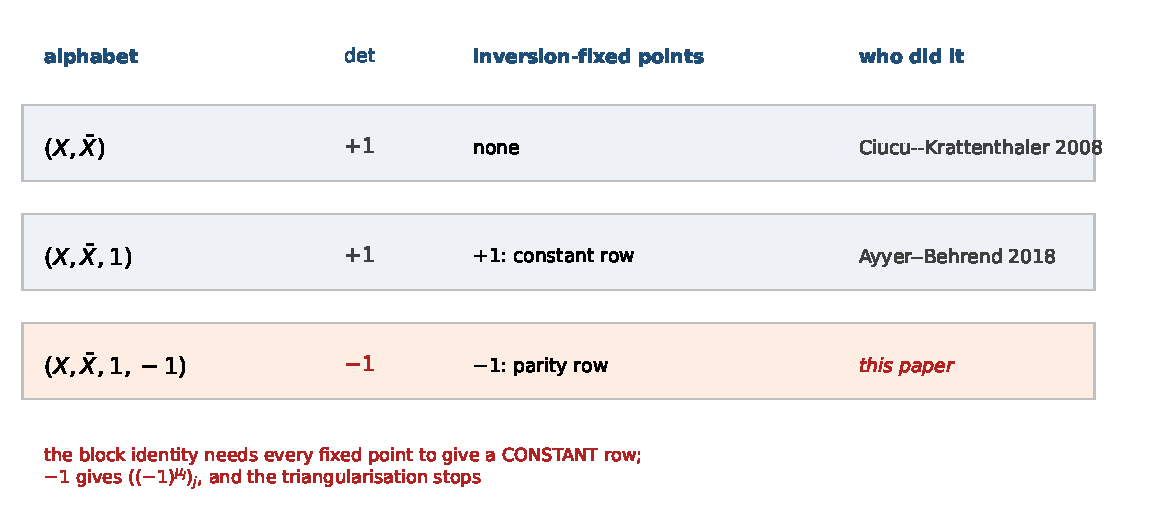
\includegraphics[width=0.94\textwidth]{fig_families.pdf}
\caption{La sucesi\'on, y el paso que nunca se dio. Cada fila es un alfabeto estable bajo
$x\mapsto x^{-1}$; la tercera columna cuenta los puntos que esa estabilidad deja fijos, porque
son los que aportan por s\'i solos una fila al bialternante. A\~nadir el primer punto fijo $+1$
no cuesta nada --- su fila es constante y el argumento de bloques la absorbe. A\~nadir el
segundo cambia el determinante del elemento de $+1$ a $-1$, es decir, lo saca de la componente
de la identidad, y su fila es un car\'acter de paridad en vez de una constante. Todo lo de este
art\'iculo es consecuencia de esa \'unica fila.}
\label{fig:families}
\end{figure}

% ===================================================================
\section{La forma cerrada}\label{sec:closedform}

Fijemos $\lambda$ con a lo sumo cuatro filas y escribamos $\mu_j=\lambda_j+4-j$ para su
$\beta$-conjunto. Separemos por paridad,
\[
E=\{j:\mu_j \text{ par}\},\qquad O=\{j:\mu_j\text{ impar}\},
\]
escribamos los $\mu_j$ pares como $2\alpha_i$ y los impares como $2\beta_i+1$, y sean
$\lambda^{(0)},\lambda^{(1)}$ las particiones de $\beta$-conjuntos $\alpha,\beta$ --- es decir,
las dos componentes del $2$-cociente de $\lambda$~\cite[Cap.~I, Ej.~1.8]{Macdonald}. Pongamos
\begin{equation}\label{eq:sign}
\zeta=(-1)^{\,\mathrm{inv}+|E|\,|O|},\qquad
\mathrm{inv}=\#\{\,i<j:\ \mu_i\ \text{impar},\ \mu_j\ \text{par}\,\},
\end{equation}
y sea $\chi_k(t)=t^k+t^{k-2}+\dots+t^{-k}$, con $\chi_{-1}=0$.

\begin{observacion}[verificada, no demostrada]\label{obs:main}
Para toda partici\'on $\lambda$ con a lo sumo cuatro filas,
\begin{equation}\label{eq:closedform}
\boxed{\;
s_\lambda(1,-1,t,t^{-1})=
\begin{cases}
0, & E=\varnothing\ \text{o}\ O=\varnothing,\\[3pt]
\zeta\,\mathrm{sgn}(z)\;
\chi_{\lambda^{(0)}_1-\lambda^{(0)}_2}\;
\chi_{\lambda^{(1)}_1-\lambda^{(1)}_2}\;
\chi_{|z|-1},
& |E|=|O|=2,\quad z=|\lambda^{(0)}|-|\lambda^{(1)}|-1,\\[3pt]
\zeta\;\chi_{\nu_1-\nu_2}\;\chi_{\nu_2-\nu_3}\;\chi_{\nu_1-\nu_3+1},
& |E|=3\ \text{o}\ |O|=3,
\end{cases}\;}
\end{equation}
donde $\nu$ denota la componente del cociente que tiene tres partes. En el caso intermedio,
$z=0$ da tambi\'en cero, a trav\'es de $\chi_{-1}=0$.
\end{observacion}

\begin{figure}[h]
\centering
\begin{tikzpicture}[x=5.0mm,y=5.0mm,line join=round]
\definecolor{evenc}{RGB}{31,78,121}\definecolor{oddc}{RGB}{178,34,34}
\definecolor{lamfill}{RGB}{205,220,236}
% lambda = (7,3,1,1) solid, staircase rho = (3,2,1,0) dashed: row length = beta
\foreach \r/\L/\S in {0/7/3, 1/3/2, 2/1/1, 3/1/0}{
  \foreach \c in {1,...,\L}{\draw[fill=lamfill,draw=evenc!70] (\c-1,-\r) rectangle ++(1,-1);}
  \ifnum\S>0 \foreach \c in {1,...,\S}{\draw[dashed,draw=black!35,fill=white]
      (\L+\c-1,-\r) rectangle ++(1,-1);}\fi}
\foreach \r/\n in {0/1,1/2,2/3,3/4}{\node[anchor=east,font=\footnotesize] at (-0.3,-\r-0.5) {$\lambda_\n$};}
\node[anchor=west,evenc,font=\footnotesize] at (10.4,-0.5) {$\beta_1=10$};
\node[anchor=west,oddc, font=\footnotesize] at (10.4,-1.5) {$\beta_2=5$};
\node[anchor=west,evenc,font=\footnotesize] at (10.4,-2.5) {$\beta_3=2$};
\node[anchor=west,oddc, font=\footnotesize] at (10.4,-3.5) {$\beta_4=1$};
\node[anchor=north,font=\footnotesize] at (5,-4.5)
  {$\lambda$ (s\'olido) $+$ escalera $\rho$ (discontinua) $=$ longitudes de fila $\beta$};
% the parity split and the three half-differences, stacked
\node[anchor=west,evenc,font=\footnotesize] at (15.6,-0.4) {$E=\{10,\,2\}$};
\node[anchor=west,evenc,font=\footnotesize] at (20.0,-0.4) {en $E$:\; $\tfrac{10-2}{2}-1=\mathbf{3}$};
\node[anchor=west,oddc, font=\footnotesize] at (15.6,-1.8) {$O=\{5,\,1\}$};
\node[anchor=west,oddc, font=\footnotesize] at (20.0,-1.8) {en $O$:\; $\tfrac{5-1}{2}-1=\mathbf{1}$};
\node[anchor=west,black!60,font=\footnotesize] at (15.6,-3.2) {$E$ vs $O$};
\node[anchor=west,black!60,font=\footnotesize] at (20.0,-3.2) {cruzado:\; $\bigl|\tfrac{12-6}{2}\bigr|-1=\mathbf{2}$};
\draw[black!25] (15.4,-4.0) -- (27.6,-4.0);
\node[anchor=west,font=\small] at (15.6,-4.8) {$D(t)\;=\;-\,\chi_{1}\,\chi_{2}\,\chi_{3}$};
\end{tikzpicture}
\caption{Los tres espines, le\'idos de un solo diagrama. Al adosar la escalera
$\rho=(3,2,1,0)$ a $\lambda=(7,3,1,1)$, las longitudes de fila pasan a ser el $\beta$-conjunto
$\beta=(10,5,2,1)$. Partir $\beta$ por paridad da $E$ y $O$; las dos semidiferencias
\emph{dentro de clase} y la \emph{cruzada}, cada una menos uno, son los tres espines $(3,1,2)$, y
\eqref{eq:sign} fija el signo. En ning\'un punto entra hip\'otesis alguna sobre la forma de
$\lambda$.}
\label{fig:readoff}
\end{figure}

As\'i que el car\'acter es siempre $\pm$ un producto de exactamente tres caracteres de $SU(2)$,
o cero (Figura~\ref{fig:readoff}), y --- este es el punto en el que merece la pena detenerse --- \textbf{no hay hip\'otesis
alguna sobre la forma de $\lambda$}. Ciucu--Krattenthaler y Ayyer--Behrend han de suponer
autocomplementariedad; \eqref{eq:closedform} no supone nada. Esa diferencia no es una mejora de
su teorema; es s\'intoma de un mecanismo distinto, y \S\ref{sec:why} dice de cu\'al.

\paragraph{Por qu\'e tres, y por qu\'e $SU(2)$.} El alfabeto tiene un solo par\'ametro libre,
as\'i que sea cual sea la respuesta, es un polinomio de Laurent en una variable, sim\'etrico
bajo $t\mapsto t^{-1}$ --- es decir, un car\'acter virtual de $SU(2)$. El contenido de
\eqref{eq:closedform} es que nunca es meramente virtual y nunca irreducible m\'as all\'a de
tres factores: dos de los tres provienen por separado de las dos componentes del cociente, y el
tercero es un t\'ermino \emph{cruzado} que mide cu\'anto se apartan en tama\~no las dos
componentes.

\paragraph{Flanco abierto: por qu\'e tres, y qu\'e es el tercer factor.} Los dos primeros
factores tienen un due\~no obvio --- uno por componente del $2$-cociente --- y el tercero no.
Depende s\'olo de $|\lambda^{(0)}|-|\lambda^{(1)}|$, y es el que produce la segunda rama de
ceros. Esa dependencia es ya una pista de d\'onde vive: un desequilibrio no es propiedad de
ninguna de las dos componentes sino del \emph{acoplamiento} entre ellas, de modo que si el
tercer factor est\'a ligado a algo, lo est\'a a eso, y no a $\lambda^{(0)}$ o
$\lambda^{(1)}$ por separado. Tres preguntas que el lector tiene derecho a hacer, ninguna de las cuales sabemos
responder.
\emph{(i)} \textquestiondown Es el tercer factor el car\'acter de un espacio de multiplicidad?
Si la restricci\'on a la clase lateral se descompone como
$\mathrm{Tr}\big(\sigma\mid V_{j_L}\otimes V_{j_R}\otimes M\big)$ con $M$ portando el
desequilibrio, la identidad dejar\'ia de ser combinatoria y pasar\'ia a ser un teorema de
ramificaci\'on, y $\mathrm{Spin}(4)=SU(2)_L\times SU(2)_R$ hace tentadora esa lectura.
\emph{(ii)} \textquestiondown Es el n\'umero tres igual a $2n-1$ en rango $n$? En rango uno eso
se lee $3=2\cdot2-1$, dos componentes del cociente y un t\'ermino cruzado, y predice cinco
factores en rango dos --- lo que \S\ref{sec:ranktwo} muestra falso en general, de modo que si
el patr\'on sobrevive, sobrevive en una subfamilia. \textquestiondown Cu\'al?
\emph{(iii)} \textquestiondown Hay demostraci\'on biyectiva? Cada $\chi_k$ tiene coeficientes
unidad, luego $\delta(m)$ cuenta puntos reticulares; una biyecci\'on entre esos puntos y algo
ligado a $\lambda$ explicar\'ia la f\'ormula en lugar de verificarla.

\paragraph{Cuatro grados de afirmaci\'on, y cu\'al es cu\'al.} Este art\'iculo mezcla teoremas
prestados, una identidad no demostrada, cosas que se siguen de ella y cosas que s\'olo
sospechamos. Confundirlas ser\'ia la forma m\'as f\'acil de enga\~nar, as\'i que se grad\'uan
una vez, aqu\'i.

\begin{center}\small
\setlength{\tabcolsep}{4pt}
\begin{tabular}{@{}l l p{5.6cm}@{}}
\toprule
\rowcolor{hdrblue}\textcolor{white}{grado} & \textcolor{white}{qu\'e significa} &
\textcolor{white}{instancias}\\
\midrule
\textbf{Proposici\'on} & demostrado, con independencia de todo lo dem\'as &
Prop.~\ref{cor:Z} (v\'ia Parte~III); ambas suficiencias, que son folclore\\
\rowcolor{softgrey}
\textbf{Observaci\'on} & verificado exhaustivamente, \emph{sin demostraci\'on} &
\eqref{eq:closedform}, la forma cerrada\\
\textbf{Heredado} & cl\'asico, citado, no nuestro &
\eqref{eq:moments}, \eqref{eq:deltaclosed}, la log-concavidad\\
\rowcolor{softgrey}
\textbf{Abierto} & sospechado, con una sonda enunciada &
el sentido del tercer factor, el rango dos, el origen del signo\\
\bottomrule
\end{tabular}
\end{center}

\noindent Enunciamos la Observaci\'on~\ref{obs:main} como verificada y no como
teorema, y la distinci\'on es intencionada. Se ha comprobado exhaustivamente con dos
implementaciones independientes --- una que deriva el cociente mediante el propio $2$-cociente
de Sage, otra que rederiva $\alpha$ y $\beta$ directamente de $\mu$, de modo que un error de
convenio en cualquiera de las dos se ver\'ia --- en las $3060$ particiones con cuatro partes
$\le14$ y en las $4845$ con cuatro partes $\le16$, frente a evaluaciones de Jacobi--Trudi en
aritm\'etica exacta de Laurent con enteros. No hubo discrepancias. No hay demostraci\'on.

% ===================================================================
\section{El lugar de ceros es la clase de la Parte III}\label{sec:zero}

Leer d\'onde se anula \eqref{eq:closedform} da dos ramas, y son las dos cl\'ausulas del Teorema
de la Parte~III: $E$ u $O$ vac\'io es la afirmaci\'on de que los cuatro $\beta$-n\'umeros
comparten paridad, y en coordenadas de $\lambda$ eso es
$\lambda_1\not\equiv\lambda_2\not\equiv\lambda_3\not\equiv\lambda_4$; y $z=0$ en la rama
equilibrada es $|\lambda^{(0)}|=|\lambda^{(1)}|+1$, que es $\lambda$ autocomplementaria ---
$\lambda_i+\lambda_{5-i}$ constante --- con esa constante impar.

\begin{proposicion}[demostrada de forma independiente en la Parte~III]\label{cor:Z}
El car\'acter se anula exactamente en
\begin{equation}\label{eq:zerolocus}
\boxed{\;
D\equiv0
\iff
\underbrace{\lambda_1\not\equiv\lambda_2\not\equiv\lambda_3\not\equiv\lambda_4}_{\text{paridad alternante}}
\quad\text{o}\quad
\underbrace{\lambda_i+\lambda_{5-i}=c\ \ \forall i,\ \ c\ \text{impar}}_{\text{autocomplementaria, constante impar}}\;}
\end{equation}
Esta es la clase $\mathcal Z$ de la Parte~III. Los dos mecanismos de anulaci\'on de
\eqref{eq:closedform} --- una clase de paridad vac\'ia, o un $2$-cociente equilibrado cuyo
\'indice cruzado $z$ degenera --- son disjuntos, aunque las dos abreviaturas en $\lambda$ del
recuadro no sean mutuamente excluyentes tal como est\'an escritas.
\end{proposicion}

\paragraph{Atribuci\'on a\~nadida en la versi\'on~3.}
La primera rama no es nuestra. Poner $t=1$ env\'ia nuestro alfabeto al elemento de orden~2
$(1,-1,1,1)$, y nuestro lema de rigidez ($D\equiv0$ exactamente cuando $D(1)=0$) lleva el criterio
de ida y vuelta. Karmakar~\cite{Karmakar}, Thm.~1A, enuncia precisamente ese criterio para
$\mathrm{GL}(n,\mathbb{C})$ en $C_{n-k,k}$: su $\eta_i(\lambda)$ es nuestro corte de paridad de
$\lambda+\rho$, y su normalizaci\'on ``$\#\eta_0\ge\#\eta_1$ tras torcer por el car\'acter
determinante'' es nuestro twist de determinante. Su Thm.~1B va m\'as lejos y factoriza el valor en
ese elemento a trav\'es del $2$-cociente, constante incluida --- la sombra en $t=1$ de
\eqref{eq:closedform}. Lo que queda espec\'ifico de este art\'iculo es la segunda rama y, sobre
todo, la evaluaci\'on con $t$ \emph{libre}. Ese programa est\'a vivo: Nadimpalli--Pattanayak--Prasad~\cite{NPP}
generalizan~\cite{Karmakar} a elementos de torsi\'on y plantean, como pregunta del tercer autor,
exactamente esta forma: anulaci\'on cuando una dimensi\'on de centralizador excede a otra, y una
constante por una \emph{dimensi\'on} cuando coinciden. Nuestro punto $t=1$ es un caso suyo. La
deformaci\'on fuera de ese punto no lo es: su programa no tiene par\'ametro libre ni componente no
identidad. (Lo comprobamos y registramos el negativo: $s_\lambda(1,-1,t,t^{-1})$ \emph{no} es $\pm$
una constante por $s_{\lambda^{(0)}}(1,t,t^{-1})$ --- $0$ de $105$ casos --- de modo que el objeto
con $t$ libre no es sin m\'as el car\'acter de la representaci\'on del centralizador cuya dimensi\'on
calcula el Thm.~1B de Karmakar.)

\paragraph{Por qu\'e es proposici\'on y no corolario.} El enunciado no depende de la
Observaci\'on~\ref{obs:main}. La Parte~III demuestra la clasificaci\'on por otra v\'ia y la
certifica en Lean, de modo que se sostiene pase lo que pase con \eqref{eq:closedform}. Lo que
aporta la forma cerrada no es el hecho sino la \emph{causa}: exhibe $\mathcal Z$ como el lugar
donde el producto degenera, y lo hace \emph{condicionada a una identidad que no hemos
demostrado}. Deducir un teorema ya demostrado a partir de una observaci\'on no demostrada no
asciende a la observaci\'on; s\'olo vuelve condicional la deducci\'on, y conviene decir en
qu\'e direcci\'on corre la l\'ogica. Quien rechace \eqref{eq:closedform} conserva entera la
Proposici\'on~\ref{cor:Z} y s\'olo pierde la explicaci\'on.

\paragraph{Flanco abierto: \textquestiondown est\'a forzada la dicotom\'ia?} Podemos decir que
no hay tercera rama; no podemos decir por qu\'e no podr\'ia haberla. En la forma cerrada las
dos ramas son visiblemente especies distintas --- una mata el producto entero vaciando una
clase de paridad, la otra mata un solo factor degenerando su \'indice --- y el lector puede
preguntar con raz\'on si eso es una dicotom\'ia genuina o un artefacto del rango uno. Dos
sondas lo zanjar\'ian. \emph{\textquestiondown Hay una dualidad que intercambie las ramas?}
Ambas son invariantes bajo conjugaci\'on compuesta con complementaci\'on en un rect\'angulo
adecuado, lo cual es sugerente y no lo hemos perseguido. \emph{\textquestiondown Y aparece una
tercera rama en rango dos?} S\'i: \S\ref{sec:ranktwo} exhibe una partici\'on que se anula con
ambas clases de paridad ocupadas, que no es ninguna de nuestras dos causas. De modo que la
dicotom\'ia es un enunciado de rango uno, y llamarla hecho estructural ser\'ia excederse.

La descomposici\'on es exacta y no deja nada. De las $560$ particiones que se anulan en el
intervalo $\text{partes}\le16$, $420$ caen en la primera rama y $140$ en la segunda, y ninguna
fuera de las dos (Figura~\ref{fig:zerolocus}).

\begin{figure}[h]
\centering
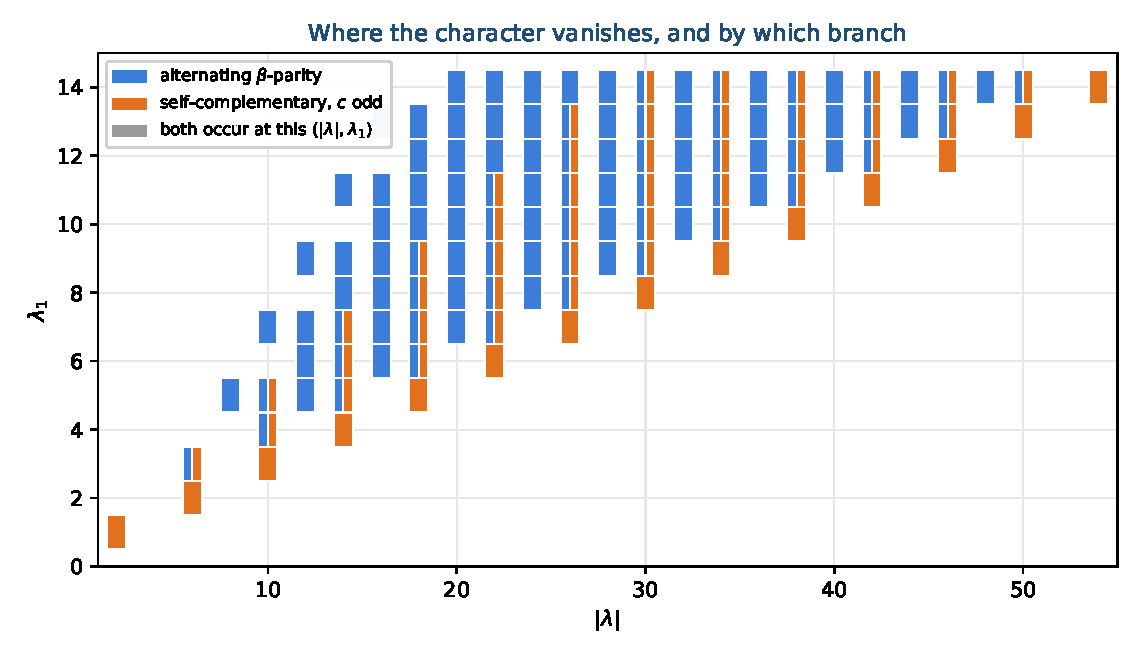
\includegraphics[width=0.86\textwidth]{fig_zerolocus.pdf}
\caption{El lugar de ceros, dibujado por tama\~no y primera parte. Las celdas azules contienen
una partici\'on matada por $\beta$-paridad alternante, las naranjas una matada por
autocomplementariedad con constante impar, las partidas ambas. El contenido de la l\'amina es
lo que \emph{no} hay en ella: no hay un tercer color. Toda partici\'on en la que
$s_\lambda(1,-1,t,t^{-1})$ se anula queda explicada por una de las dos ramas, que es lo que
significa que la Proposici\'on~\ref{cor:Z} sea exhaustiva y no meramente correcta.}
\label{fig:zerolocus}
\end{figure}

\paragraph{Una direcci\'on de suficiencia es folclore y no la reclamamos.} Que la
autocomplementariedad con constante impar fuerce la anulaci\'on son dos l\'ineas y no es nuevo:
escribiendo $\lambda^\star_i=c-\lambda_{5-i}$ se tiene $s_{\lambda^\star}(x)=(x_1\cdots x_4)^c
s_\lambda(x^{-1})$; nuestro alfabeto es estable por inversi\'on, luego
$s_\lambda(p^{-1})=s_\lambda(p)$; y $x_1\cdots x_4=\det=-1$. Si $\lambda^\star=\lambda$
entonces $s_\lambda(p)=(-1)^cs_\lambda(p)$, y $c$ impar fuerza cero. Esta es la sombra, en
funciones de Schur, del enunciado de manual de que una irreducible autoasociada de $O(n)$
satisface $V\cong V\otimes\det$ y por tanto tiene car\'acter nulo fuera de
$SO(n)$~\cite[Cap.~XI, \S11.6, \S11.8]{LittlewoodBook}. La otra rama es igual de elemental: la
igualdad de paridad de todos los $\beta$-n\'umeros hace proporcionales las filas del
bialternante en $x=1$ y $x=-1$. \textbf{Lo que se reclama aqu\'i es la forma cerrada, no
ninguna de las dos suficiencias.}

% ===================================================================
\section{Lo que los ceros escond\'ian}\label{sec:moments}

La Proposici\'on~\ref{cor:Z} responde a la pregunta que hizo la Parte~III. No es la pregunta que la
Parte~III necesitaba que se respondiera.

La dificultad de aquel art\'iculo empezaba \emph{despu\'es} de la anulaci\'on: habiendo
mostrado que la contribuci\'on fermi\'onica dominante a la curvatura de la l\'inea de Wilson se
cancela id\'enticamente para toda representaci\'on admisible, no quedaba sino comparar
representaciones por lo que sobrevive, y lo que sobrevive no lo gobierna si $\delta(m)$ se
anula sino sus \emph{momentos}. All\'i se calculaban enumerando el sistema de pesos de cada
irreducible de $\su4$ peso a peso. La forma cerrada elimina esa enumeraci\'on por completo, y
lo hace por una raz\'on que se ve en cuanto uno la escribe.

Los coeficientes de $D$ son los desequilibrios de twist, $\delta(m)=[t^m]D(t)$. Si
$D=\zeta\,\chi_p\chi_q\chi_r$ entonces $\delta$ es la \emph{convoluci\'on triple} de tres
caracteres, es decir, $\delta(m)$ cuenta, con un signo global, las soluciones de
\begin{equation}\label{eq:convolution}
m=(p-2i)+(q-2j)+(r-2k),\qquad 0\le i\le p,\ 0\le j\le q,\ 0\le k\le r .
\end{equation}
Todo $\chi_k$ es sim\'etrico bajo $m\mapsto-m$, luego todos los momentos impares se anulan y
--- esto es lo que hace corta la respuesta --- los t\'erminos cruzados de primer orden de un
producto se cancelan tambi\'en. Escribiendo $M_{2r}(f)=\sum_m m^{2r}f(m)$ y
$M_2(\chi_k)=\sum_{j=0}^{k}(k-2j)^2=\tfrac13k(k+1)(k+2)$:
\begin{equation}\label{eq:moments}
\boxed{\;
\begin{aligned}
M_0(\delta)&=\zeta\,(p{+}1)(q{+}1)(r{+}1),\\[2pt]
M_2(\delta)&=\zeta\Big[M_2(\chi_p)(q{+}1)(r{+}1)+(p{+}1)M_2(\chi_q)(r{+}1)
+(p{+}1)(q{+}1)M_2(\chi_r)\Big],
\end{aligned}\;}
\end{equation}
y $M_4$ an\'alogamente, restituyendo los t\'erminos cruzados por pares
$6\sum M_2(\chi_\bullet)M_2(\chi_\bullet)(\cdot+1)$. Toda la torre de momentos es polin\'omica
en los tres enteros $(p,q,r)$.

\paragraph{Dado $(p,q,r)$, nada de eso es nuestro.} Hab\'iamos presentado \eqref{eq:moments}
como una aportaci\'on y no lo es. La sucesi\'on de coeficientes de un producto de caracteres de
$sl_2$ es la convoluci\'on de las multiplicidades de peso, es decir, de tres sucesiones
uniformes discretas --- un diccionario escrito expl\'icitamente, con factores de Chebyshev
incluidos, por Bradley y Gupta~\cite{BradleyGupta}. Todo cumulante de una uniforme discreta de
anchura $w$ es un polinomio en $w$ con coeficientes de Bernoulli, y los cumulantes se suman
sobre sumandos independientes~\cite{Neuschel}; la polinomialidad de la torre entera sale en una
l\'inea. Lo nuestro no es la aritm\'etica sino la \emph{reducci\'on que la alimenta}: que una
partici\'on de cuatro filas entra s\'olo a trav\'es de tres enteros le\'idos de su
$2$-cociente. La Parte~III enumeraba sistemas de pesos porque no ten\'ia esa reducci\'on, no
porque las sumas fueran dif\'iciles.

\paragraph{Los momentos se organizan por Casimir.} Escribamos
\[
C_k \;=\; k(k+2)\;=\;4j(j+1),\qquad j=k/2,
\]
el Casimir cuadr\'atico de la irreducible de $SU(2)$ de peso m\'aximo $k$, y sean $e_1,e_2$ las
funciones sim\'etricas elementales de $C_p,C_q,C_r$. Dividir por $M_0$ cancela $\zeta$, de modo
que lo que sigue no lleva signo:
\begin{equation}\label{eq:casimir}
\boxed{\;
\frac{M_2(\delta)}{M_0(\delta)}=\frac{e_1}{3},
\qquad
\frac{M_4(\delta)}{M_0(\delta)}=\frac{2}{3}e_2+\frac{1}{5}\big(C_p^2+C_q^2+C_r^2\big)
-\frac{4}{15}e_1 .\;}
\end{equation}
Somos cuidadosos con lo que esto es. Como \emph{f\'ormula}, la primera identidad es cl\'asica:
es la varianza de una suma de tres uniformes discretas independientes, y la varianza de anchura
$w$ que la produce es est\'andar~\cite{Neuschel}. Lo que a\~nadimos es s\'olo la \emph{lectura}
--- que el entero $k(k+2)$ que aparece ah\'i es $4j(j+1)$, el Casimir de $sl_2$ en esp\'in
$j=k/2$, de modo que la varianza de la distribuci\'on de desequilibrios de twist es un tercio
de la suma de tres Casimires. Eso es una interpretaci\'on y no un teorema, y as\'i lo
se\~nalamos. Lo dejamos anotado igualmente porque es el \'unico lugar de este art\'iculo donde
los tres factores de \eqref{eq:closedform} se comportan como representaciones y no como tres
factores polin\'omicos convenientes, que es exactamente la pregunta que
\S\ref{sec:closedform} deja abierta.

Escrito as\'i, el patr\'on no se detiene en $M_4$, y el enunciado general es una proposici\'on y
no una conjetura, porque su demostraci\'on es media p\'agina de material cl\'asico.

\begin{proposicion}[la torre de momentos vive en un anillo de invariantes]\label{prop:ring}
Sup\'ongase la Observaci\'on~\ref{obs:main}, de modo que $\delta=\zeta\,\chi_p*\chi_q*\chi_r$.
Entonces, para todo $r\ge0$,
\[
\frac{M_{2r}(\delta)}{M_0(\delta)}\;\in\;
\mathbb{Q}\big[C_p,C_q,C_r\big]^{S_3}=\mathbb{Q}[e_1,e_2,e_3],
\]
y todos los momentos impares se anulan. El coeficiente de $e_1^{\,r}$ es $1/(2r+1)$.
\end{proposicion}

\begin{proof}
Normalizado, $\chi_k$ es la ley de $2U_k-k$ con $U_k$ uniforme en $\{0,\dots,k\}$. Sus
cumulantes impares se anulan por simetr\'ia, y por el lema de
Neuschel~\cite[Lema~2.1]{Neuschel} los pares valen
$\kappa_{2l}=4^{\,l}\frac{B_{2l}}{2l}\big((k+1)^{2l}-1\big)$. Ahora bien,
$(k+1)^2=k(k+2)+1=C_k+1$, luego $(k+1)^{2l}=(C_k+1)^l$ y
\[
\kappa_{2l}(\chi_k)=4^{\,l}\,\frac{B_{2l}}{2l}\Big[(C_k+1)^l-1\Big]\in\mathbb{Q}[C_k].
\]
Los cumulantes son aditivos sobre sumandos independientes, de modo que
$\kappa_{2l}(\delta/M_0)$ es la suma de los tres, un polinomio sim\'etrico en $C_p,C_q,C_r$;
los momentos son polinomios universales en los cumulantes; y los polinomios sim\'etricos en
tres cantidades est\'an libremente generados por $e_1,e_2,e_3$. El coeficiente principal se
sigue de $\kappa_2=C_k/3$ y de que el t\'ermino en $e_1^{\,r}$ de $M_{2r}$ es el momento
$r$-\'esimo de una \'unica contribuci\'on sin acoplar, $(2r-1)!!$ veces $\kappa_2^{\,r}$
dividido por la normalizaci\'on $(2r+1)$ de la sucesi\'on plana.\footnote{Verificado y no
derivado para $r\ge3$: la identidad se comprob\'o exactamente para $r=1,\dots,8$ en los $729$
tripletes con $p,q,r\le8$, resolviendo el sistema sobredeterminado en aritm\'etica racional
exacta. Controles: sustituir $C_k=k(k+2)$ por $k(k+3)$ vuelve el sistema inconsistente en
$r=1,2,3$, y lo mismo ocurre al suprimir la normalizaci\'on por $M_0$.}
\end{proof}

\paragraph{Por qu\'e esto no es una tautolog\'ia.} Lo ser\'ia si todo polinomio sim\'etrico en
$(p,q,r)$ fuese un polinomio en los Casimires. No lo es. Ya $p+q+r$ no lo es: poniendo $q=r=0$,
una identidad polin\'omica $p=P(C_p)$ dar\'ia $\deg_p\text{izq}=2\deg P$ frente a
$\deg_p\text{der}=1$. La aplicaci\'on
\[
(p,q,r)\;\longmapsto\;(C_p,C_q,C_r),\qquad C_k=k(k+2),
\]
\emph{olvida} el dato lineal --- $k+1=\sqrt{C_k+1}$ s\'olo se recupera a trav\'es de una ra\'iz
cuadrada --- y sin embargo la torre entera de momentos sobrevive a esa p\'erdida. El control de
arriba dice lo mismo emp\'iricamente: mu\'evase el invariante en una unidad, a $k(k+3)$, y
ning\'un polinomio ajusta a ning\'un orden.

\paragraph{El funcional f\'isico factoriza a trav\'es del $2$-cociente.} Es la forma m\'as
limpia que conocemos de decir qu\'e hace este art\'iculo, y merece enunciarse una vez as\'i. Sea
$\Phi(\lambda)=\{M_{2r}(\lambda)\}_{r\ge0}$ la torre de momentos que la Parte~III necesita, y
sea $Q(\lambda)=(p,q,r)$ los tres enteros le\'idos del $2$-cociente. Entonces, condicionada a la
Observaci\'on~\ref{obs:main},
\begin{equation}\label{eq:factorfunctional}
\boxed{\;\Phi=F\circ Q\;}
\end{equation}
para un $F$ universal que no sabe nada de $\lambda$. La factorizaci\'on en tres caracteres es el
\emph{mecanismo}; esta reducci\'on es el \emph{contenido}. Una partici\'on de cuatro filas puede
ser arbitrariamente grande, y toda cantidad que sobrevive a la cancelaci\'on dominante de la
Parte~III depende de ella a trav\'es de tres enteros y de nada m\'as.

\paragraph{Comprobado, y comprobado de modo que pudiera fallar.} En las $1612$ particiones con
cuatro partes $\le12$ en las que $D\not\equiv0$: la factorizaci\'on en tres caracteres se
hall\'o pelando el polinomio directamente y no aplicando la receta de \'indices de
\eqref{eq:closedform}, de modo que esto confirma de forma independiente que el n\'umero de
factores es tres; y $M_0$, $M_2$ y $M_4$ de \eqref{eq:moments} coincidieron con los momentos
le\'idos de $D$ en todos los casos. Como control se evalu\'o la misma f\'ormula con un
\'indice desplazado en una unidad, donde coincidi\'o en $0$ de $1612$ --- la prueba era capaz
de fallar. Las formas de Casimir \eqref{eq:casimir} se comprobaron despu\'es por dos v\'ias que
no comparten c\'odigo: una suma directa sobre la caja $(i,j,k)$, que no construye la
convoluci\'on en ning\'un momento, en los $1331$ tripletes con $p,q,r\le10$; y una evaluaci\'on
simb\'olica de $(t\,\partial_t)^{2r}$ en $t=1$ sobre $216$ tripletes. Ambas coinciden con
\eqref{eq:casimir} y entre s\'i. Controles: desplazar un \'indice coincide en $0$ de $216$, y
perturbar el coeficiente $4/15$ a $3/15$ coincide en $1$ de $216$.

\begin{figure}[htbp]
\centering
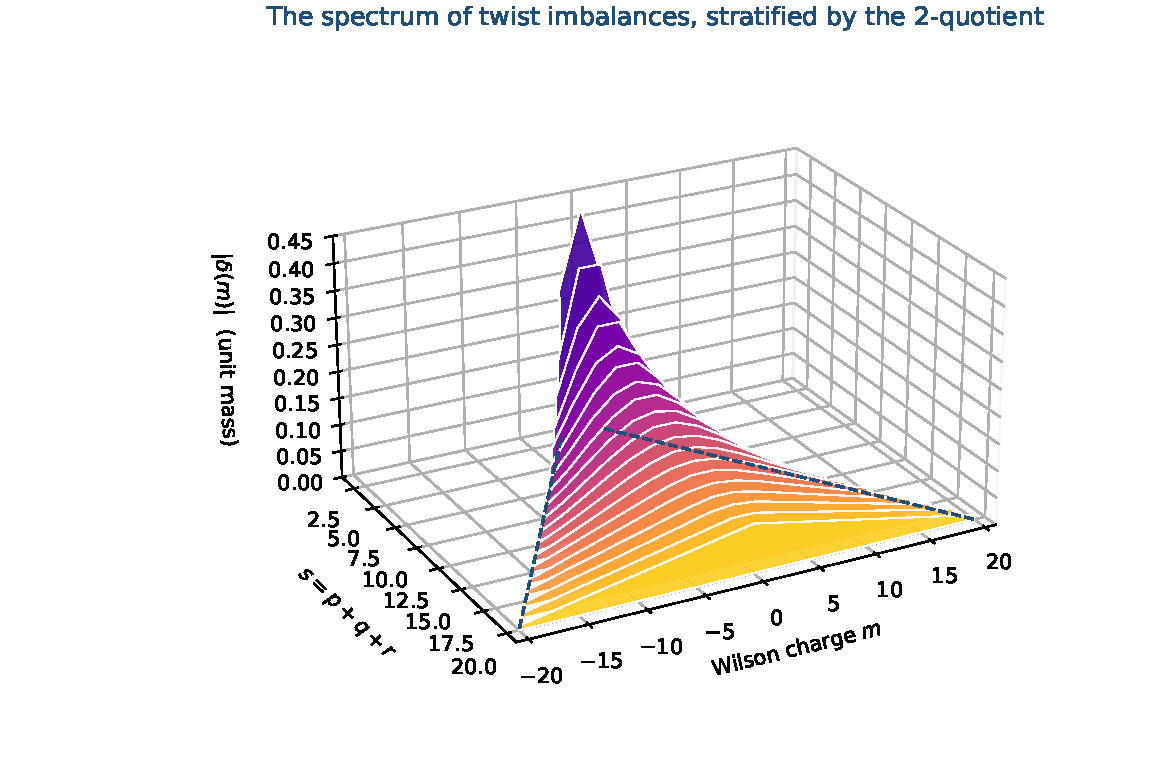
\includegraphics[width=\linewidth]{fig_spectrum3d.pdf}
\caption{El espectro de desequilibrios de twist. Cada cresta es el perfil agregado de
$|\delta(m)|$ sobre todas las particiones con cuatro partes y $|\lambda|\le20$ que comparten un
valor de $s=p+q+r$, normalizado a masa unidad para que un soporte que se ensancha tenga que
pagarlo en amplitud. Las l\'ineas discontinuas son $m=\pm s$: el contenido de la l\'amina es
que las crestas las alcanzan y se detienen, en todos los estratos, que es \eqref{eq:convolution}
le\'ida como enunciado sobre el soporte y no sobre los momentos. El flujo de pico a meseta es
la convoluci\'on haciendo lo que hacen las convoluciones, y es la forma que $M_0$, $M_2$, $M_4$
s\'olo muestrean.}
\label{fig:spectrum3d}
\end{figure}

\paragraph{La distribuci\'on misma, no s\'olo sus momentos.} El mismo diccionario da $\delta$
en forma cerrada y no s\'olo sus momentos. Con $s=p+q+r$ y $N=(s-m)/2$, $\delta(m)/\zeta$ cuenta
las soluciones de $i+j+k=N$ en la caja $0\le i\le p$, $0\le j\le q$, $0\le k\le r$, de modo que
la inclusi\'on--exclusi\'on sobre el conteo no acotado de barras y estrellas da
\begin{equation}\label{eq:deltaclosed}
\frac{\delta(m)}{\zeta}\;=\;\sum_{A\subseteq\{p,q,r\}}(-1)^{|A|}
\binom{\,N-\sum_{a\in A}(a+1)+2\,}{2}_{\!\!+},
\end{equation}
leyendo el binomio como cero cuando su argumento superior baja de $2$. Esto es
inclusi\'on--exclusi\'on de manual; el caso de cotas iguales se remonta a De~Moivre y tiene
tratamiento monogr\'afico en Andr\'e~\cite{Andre}, la familia de coeficientes es lo que Comtet
llama \emph{coeficientes polin\'omicos}~\cite[p.~77]{Comtet}, y la propia funci\'on
polin\'omica a trozos es un \emph{discrete box spline} en el sentido de Dahmen y
Micchelli~\cite{DahmenMicchelli}. No reclamamos nada de ello. Lo enunciamos porque asciende el
soporte --- que la Figura~\ref{fig:spectrum3d} comprueba estrato a estrato --- de observaci\'on
verificada a consecuencia inmediata, y porque permite sustituir $\delta(m)$ directamente en una
suma de Coleman--Weinberg en vez de tabularla.

\paragraph{Para qu\'e sirve.} $M_2(\delta)$ es precisamente la cantidad que gobierna qu\'e
sector domina la curvatura del potencial de la l\'inea de Wilson en el escenario de la
Parte~III, donde aparec\'ia como un n\'umero extra\'ido de una enumeraci\'on de pesos y no
llevaba estructura. Aqu\'i es un polinomio c\'ubico en tres enteros le\'idos del $2$-cociente.
La identidad de \S\ref{sec:closedform} no es por tanto s\'olo un hecho sobre funciones
sim\'etricas: es el asidero anal\'itico para los t\'erminos subdominantes que la Parte~III
pod\'ia describir pero no calcular.

\paragraph{Flanco abierto: \textquestiondown qu\'e m\'as delata una convoluci\'on?} Una
convoluci\'on triple de sucesiones sim\'etricas con coeficientes unidad es un objeto muy
constre\~nido, y no hemos usado casi nada de eso. Una pregunta que hac\'iamos aqu\'i en un
borrador anterior --- \emph{\textquestiondown es $|\delta|$ log-c\'oncava, o unimodal?} --- no
era una pregunta en absoluto, y la correcci\'on va en el texto y no en una nota al pie. Cada
$\chi_k$, restringido a la clase de paridad que ocupa, es la sucesi\'on constante
$(1,1,\dots,1)$, que es log-c\'oncava y sin ceros internos; la log-concavidad se preserva bajo
convoluci\'on~\cite{Hoggar}, y una sucesi\'on log-c\'oncava sin ceros internos es
unimodal~\cite{Stanley}. As\'i que $|\delta|$ es sim\'etrica, sin huecos en su clase de
paridad, log-c\'oncava y unimodal, por teoremas de 1974 y 1989. Verificamos las cuatro
propiedades en $3375$ tripletes antes de encontrar las referencias, que es el orden equivocado
y es la raz\'on de que lo tuvi\'eramos archivado como abierto.
\emph{\textquestiondown Cu\'al es el soporte?} Es
$[-(p{+}q{+}r),\,p{+}q{+}r]$ con huecos de dos, luego la mayor carga de Wilson que porta
desequilibrio es $p+q+r$, un entero le\'ido del $2$-cociente. Combinatoriamente eso est\'a
zanjado --- la Figura~\ref{fig:spectrum3d} lo comprueba en todos los estratos hasta $s=20$ y la
comprobaci\'on es una aserci\'on en el script que la dibuja, de modo que un contraejemplo
impedir\'ia que la figura llegara a trazarse. Lo que \emph{no} hemos hecho es confrontarlo con
los espectros f\'isicos, donde es una predicci\'on falsable que cabe en una l\'inea: ninguna carga de
Wilson por encima de $p+q+r$ porta desequilibrio alguno. \emph{\textquestiondown Y qu\'e
significa $\zeta$?} Fija a la vez el signo de todos los momentos, luego decide la
\emph{direcci\'on} de la contribuci\'on fermi\'onica a la curvatura. Que un signo de
ordenaci\'on de un $\beta$-conjunto decida el signo de una curvatura f\'isica es o una
coincidencia de contabilidad o la sombra de algo, y no sabemos distinguirlo.

Somos cuidadosos con el estatus. \eqref{eq:moments} es consecuencia de la
Observaci\'on~\ref{obs:main} y hereda su estatus exactamente: verificada, no demostrada. Lo que
es independiente de ese estatus es la forma de \eqref{eq:convolution} --- \emph{si} el car\'acter
factoriza en tres, \emph{entonces} los momentos son polin\'omicos --- y esa implicaci\'on es
elemental.

% ===================================================================
\section{Por qu\'e no estaba ya disponible}\label{sec:why}

La obstrucci\'on es una \'unica hip\'otesis no enunciada, y localizarla es m\'as \'util que la
identidad.

El argumento de Ayyer--Behrend alcanza \eqref{eq:blockid} porque todo punto fijo de la
inversi\'on del alfabeto aporta una fila del bialternante que es \emph{constante} en el
\'indice de columna. Para el punto fijo $+1$ esa fila es $(1,1,\dots,1)$, y una fila constante
sobrevive a la operaci\'on de columnas ``restar la derecha de la izquierda'' como un bloque
uniformemente nulo, que es lo que preserva la triangularidad; su Teorema~3 trata el $1$ extra
de $(X,\bar X,1)$ exactamente sobre esa base.

El segundo punto fijo $-1$ aporta
\begin{equation}\label{eq:parityrow}
\big((-1)^{\mu_j}\big)_j,
\end{equation}
un car\'acter de paridad del \'indice de columna, y \eqref{eq:parityrow} no es constante. Bajo
la misma operaci\'on de columnas sus entradas pasan a ser $(-1)^{\mu_j}-(-1)^{\mu_{j'}}$, que
es $0$ o $\pm2$ seg\'un la paridad relativa de $\mu_j$ y $\mu_{j'}$; el bloque no
triangulariza, y el argumento se detiene. Peor a\'un, en su normalizaci\'on los exponentes son
semienteros, donde $(-1)^{\text{semientero}}$ no est\'a definido en absoluto --- una salvedad
que ellos mismos enuncian~\cite[p.~3]{AB}. As\'i que el alfabeto no est\'a meramente sin tratar
en ese marco; en ese marco no se puede ni escribir.

Hay una forma m\'as afilada de decir lo mismo. La fila \eqref{eq:parityrow} impone una
partici\'on de las \emph{columnas} por la paridad de $\mu_j$. La hip\'otesis de
autocomplementariedad impone una partici\'on distinta de las columnas, en las dos mitades de un
$\beta$-conjunto sim\'etrico. La maquinaria de bloques s\'olo puede respetar una de las dos a la vez.

\paragraph{La reparaci\'on.} Sustit\'uyanse las dos filas de puntos fijos $(1)_j$ y
$\big((-1)^{\mu_j}\big)_j$ por las filas indicadoras de las clases de paridad,
\begin{equation}\label{eq:repair}
\begin{pmatrix}1&1\\1&-1\end{pmatrix}:\qquad
\big(1\big)_j,\ \big((-1)^{\mu_j}\big)_j\ \longmapsto\
2\cdot\big(\mathbf 1_{\mu_j\,\mathrm{par}}\big)_j,\ 2\cdot\big(\mathbf 1_{\mu_j\,\mathrm{impar}}\big)_j,
\end{equation}
un cambio de base que cuesta un factor $-\tfrac12$. Las dos filas son ahora filas indicadoras
de una partici\'on de columnas, de modo que el desarrollo de Laplace por ellas es una suma
sobre una columna par y una impar, y el menor residual es el determinante de bloques de pares
rec\'iprocos sobre las columnas que quedan. Este es el an\'alogo del Teorema~3 de
Ayyer--Behrend para el segundo punto fijo.

En rango uno --- un par rec\'iproco, nuestro caso --- el menor residual es $2\times2$ y vale
$t^{\,\mu_c-\mu_d}-t^{-(\mu_c-\mu_d)}$, un \'unico car\'acter para cada elecci\'on de columnas.
Por eso \eqref{eq:closedform} no necesita hip\'otesis sobre $\lambda$: no queda nada que una
condici\'on de forma pueda constre\~nir.

\paragraph{Flanco abierto: \textquestiondown es la condici\'on de fila constante la
obstrucci\'on, o un s\'intoma?} Hemos identificado d\'onde se detiene el argumento est\'andar,
que no es lo mismo que saber por qu\'e nadie fue m\'as all\'a. Compiten dos lecturas. En la
primera es t\'ecnica: la reparaci\'on \eqref{eq:repair} muestra que se puede rodear, y el caso
qued\'o intacto s\'olo porque nadie tuvo motivo para escribir un $-1$ junto a un par
rec\'iproco --- el nuestro vino de una proyecci\'on de orbifold, no de dentro del tema. En la
segunda es estructural: $+1$ y $-1$ difieren en estar en componentes distintas de $O(n)$, y un
argumento que nunca abandona la componente de la identidad no tiene raz\'on para desarrollar
maquinaria para la que s\'i la abandona. Las dos lecturas hacen predicciones distintas para
$\mu_t$ con $t>2$, donde aparecen varios puntos fijos a la vez, y ah\'i es donde mirar\'iamos
para decidir entre ellas.

% ===================================================================
\section{Rango dos, donde paramos}\label{sec:ranktwo}

En rango dos los menores residuales son $4\times4$ sobre un subconjunto arbitrario de cuatro
columnas, y \eqref{eq:blockid} se aplica a tal menor s\'olo cuando el conjunto de columnas
superviviente es a su vez sim\'etrico. En la suma de Laplace aparecen muchos subconjuntos y
no pueden ser todos sim\'etricos a la vez, de modo que el resultado gen\'erico es una suma de
productos y no un producto. No es, sin embargo, uniformemente negativo --- que es precisamente
por lo que esto es una frontera y no un muro:

\begin{center}\small
\begin{tabular}{lp{9.4cm}}
\toprule
\rowcolor{hdrblue}
\textcolor{white}{$\lambda$ en rango dos} & \textcolor{white}{$s_\lambda(1,-1,a,\bar a,b,\bar b)$}\\
\midrule
$(2,2,2,0,0,0)$ & $\big(a^2b^2+a^2+ab+b^2+1\big)^2/(ab)^2$ --- un cuadrado perfecto: la
factorizaci\'on sobrevive\\
\rowcolor{softgrey}
$(2,2,1,1,0,0)$ & $-(a^2{-}a{+}1)(a^2{+}a{+}1)(b^2{-}b{+}1)(b^2{+}b{+}1)/(ab)^2$ --- se parte en
piezas de rango uno\\
$(3,3,1,1,0,0)$ & $-(a^2{+}1)(b^2{+}1)\cdot(\text{irreducible de bigrado }(4,4))/(ab)^3$ --- \emph{no}
se parte\\
\rowcolor{softgrey}
$(3,2,2,1,1,0)$ & $0$ --- y ambas clases de paridad son no vac\'ias\\
\bottomrule
\end{tabular}
\end{center}

Las cuatro filas se recalcularon a partir del bialternante $6\times6$ y se factorizaron sobre
$\mathbb{Q}[a,b]$ en aritm\'etica exacta con SageMath. Merece decirse porque la tercera fila
estaba mal en un borrador anterior: su factor restante es irreducible, pero tiene grado $4$ en
cada variable y grado total $8$, no grado $4$. Un grado es una afirmaci\'on como cualquier otra.

La \'ultima fila es lo m\'as afilado que podemos decir sobre el rango dos: la regla de
anulaci\'on all\'i es \emph{estrictamente m\'as fina} que ``ambas clases de paridad
ocupadas'', que es la regla entera en rango uno. Lo que la gobierne no se ve desde este lado.

\paragraph{Flanco abierto: \textquestiondown qu\'e habr\'ia que buscar en rango dos?}
Sospechamos que el objetivo honesto no es un producto. Si la suma de Laplace se organiza por
qu\'e columnas sobreviven, la forma natural es
\[
s_\lambda(1,-1,X,\bar X)\;=\;\sum_\eta \epsilon_\eta\,
\chi^{\,\mathrm{Sp/O}}_{\alpha_\eta}(X)\,\chi^{\,\mathrm{Sp/O}}_{\beta_\eta}(X),
\]
una \emph{suma con signo} sobre selecciones compatibles con el $2$-cociente, que colapsa a un
solo t\'ermino en rango uno. Bajo esa lectura el cuadrado perfecto en $(2,2,2,0,0,0)$ es una
recombinaci\'on y no una factorizaci\'on, y el cero extra en $(3,2,2,1,1,0)$ es una cancelaci\'on
\emph{entre} t\'erminos y no la anulaci\'on de un factor --- lo que explicar\'ia por qu\'e el
criterio de rango uno deja de controlarlo. No hemos derivado el conjunto de \'indices $\eta$, y
hasta que alguien lo haga, la frase ``la factorizaci\'on a veces sobrevive'' debe leerse como
descripci\'on de resultados y no como enunciado sobre el mecanismo.

% ===================================================================
\section{El signo}\label{sec:sign}

Tres mecanismos distintos producen signos en esta literatura y no deben confundirse: un
$\mathrm{sgn}$ de una permutaci\'on de ordenaci\'on (el $(-1)^{n(n-1)/2}$ de Ayyer--Behrend
procedente de la inversi\'on de columnas, que se cancela contra su denominador); un
$(-1)^{\sum\lambda_i}$ que es artefacto de enunciar el miembro derecho en $-x$ y no en \'indice
semientero (su Ec.~(8)); y el $\mathrm{sgn}(\sigma_\lambda)$ de la permutaci\'on que ordena un
$\beta$-conjunto por clase de residuo, que es el que aparece en la l\'inea de ra\'ices de la
unidad.

El nuestro es del tercer tipo. El $\zeta$ de \eqref{eq:sign} es funci\'on del patr\'on de
paridad del $\beta$-conjunto y de nada m\'as: $(-1)^{\mathrm{inv}}$ es el signo de la
permutaci\'on que ordena $\mu$ en pares-luego-impares preservando el orden relativo, y
$(-1)^{|E||O|}$ es la constante que lo acompa\~na. \emph{No} es un $(-1)^{|\lambda|}$.

\paragraph{Una correcci\'on que le debemos al lector.} En una primera pasada registramos el
signo como si cambiara con la anchura del rect\'angulo $c$, habiendo tabulado representantes
que casualmente coincid\'ian con esa lectura. No es as\'i: ya dentro de $c=6$, $(6,6,0,0)$ y
$(4,4,2,2)$ dan $+$ mientras que $(5,5,1,1)$ y $(3,3,3,3)$ dan $-$. Para la familia
$\lambda=(a,a,b,b)$ la regla es $(-1)^{\lambda_1}$. El invariante estaba en los datos; el
muestreo no.

\paragraph{Flanco abierto.} Que el signo sea de \emph{ordenaci\'on} y no una paridad de peso no
es un detalle de contabilidad. Un $(-1)^{|\lambda|}$ dir\'ia que al objeto le importa el
tama\~no de $\lambda$; $\mathrm{sgn}(\sigma_\lambda)$ dice que le importa el orden en que el
$\beta$-conjunto se separa en clases de residuo, que es el invariante que gobierna el programa
de ra\'ices de la unidad en $t=2$. Si alguna vez se demuestra la forma cerrada por una v\'ia
que pase por ese programa y no por el bialternante, el signo es donde las dos versiones
tendr\'an que coincidir, y es por tanto la comprobaci\'on de consistencia m\'as barata
disponible sobre cualquier demostraci\'on propuesta.

% ===================================================================
\section{Libro de cuentas}\label{sec:ledger}

\begin{table}[h]
\centering\small
\begin{tabular}{p{4.0cm}p{5.2cm}p{5.0cm}}
\toprule
\rowcolor{hdrblue}
\textcolor{white}{Elemento} & \textcolor{white}{Heredado (cita)} & \textcolor{white}{Nuestro}\\
\midrule
el alfabeto como elemento de $O(4)^-$ &
elemental; cierre por inversi\'on y $\det=-1$ &
nada\\
\midrule
\rowcolor{softgrey}
autoasociada $\Rightarrow$ el car\'acter se anula fuera de $SO(n)$ &
Littlewood~\cite[Cap.~XI]{LittlewoodBook}; Weyl~\cite{Weyl} &
nada --- renunciamos a esta suficiencia expl\'icitamente\\
\midrule
igual $\beta$-paridad $\Rightarrow$ anulaci\'on &
elemental (dos filas proporcionales del bialternante) &
presentado como observaci\'on, no como resultado\\
\midrule
\rowcolor{softgrey}
la identidad de bloques \eqref{eq:blockid} y su uso &
Ayyer--Behrend~\cite{AB} Ec.~(23), Tma.~1, Tma.~3; Ciucu--Krattenthaler~\cite{CK} &
nada --- tomamos prestado el motor y decimos d\'onde se cala\\
\midrule
$t$-n\'ucleo / $t$-cociente gobernando la anulaci\'on en $\omega^kX$ &
Ayyer--Kumari~\cite{AK}, Kumari~\cite{Kumari}, Albion~\cite{Albion},
Karmakar~\cite{Karmakar} &
\textbf{correcci\'on v3:} el Thm.~1A de Karmakar \emph{es} la primera rama de
nuestro criterio de anulaci\'on, y su Thm.~1B es la factorizaci\'on por
$2$-cociente en $t=1$; s\'olo la $t$ libre es nuestra\\
\midrule
\rowcolor{softgrey}
la forma cerrada \eqref{eq:closedform} & --- &
nuestra, y \emph{verificada, no demostrada}\\
\midrule
la reparaci\'on del par de puntos fijos \eqref{eq:repair} & --- & nuestra\\
\midrule
\rowcolor{softgrey}
Proposici\'on~\ref{cor:Z} (el lugar de ceros) & la Parte~III~\cite{PartIII} demuestra la
clasificaci\'on sin condiciones & la identificaci\'on de \'esta como lugar de ceros,
condicionada a \eqref{eq:closedform}\\
\midrule
la torre de momentos \eqref{eq:moments}, dado $(p,q,r)$ &
los cumulantes de uniformes discretas son polin\'omicos en la anchura y se
suman~\cite{Neuschel}; el diccionario car\'acter/convoluci\'on~\cite{BradleyGupta} &
nada --- s\'olo la reducci\'on $\lambda\mapsto(p,q,r)$ que la alimenta\\
\midrule
\rowcolor{softgrey}
$\delta$ en forma cerrada \eqref{eq:deltaclosed}, la log-concavidad &
inclusi\'on--exclusi\'on de manual; Andr\'e~\cite{Andre}, Comtet~\cite{Comtet},
Dahmen--Micchelli~\cite{DahmenMicchelli}; Hoggar~\cite{Hoggar}, Stanley~\cite{Stanley} &
nada --- hab\'iamos confundido un teorema cl\'asico con una pregunta abierta\\
\midrule
la lectura por Casimires \eqref{eq:casimir} & la f\'ormula es la varianza
cl\'asica~\cite{Neuschel} & la lectura de $k(k+2)$ como $4j(j+1)$; interpretaci\'on, no
teorema\\
\bottomrule
\end{tabular}
\caption{Lo que debe cada elemento. La novedad aqu\'i es una identidad y un cambio de base;
todo mecanismo en el que se apoya es prestado y citado.}
\label{tab:ledger}
\end{table}

\paragraph{D\'onde miramos.} Por f\'ormula y por estructura, y no por nuestro propio
vocabulario: \emph{self-complementary partition in a rectangle character factorization};
\emph{factorization theorem classical group characters plane partitions}; \emph{Schur function
at $(x,\bar x,1)$ product of orthogonal and symplectic characters}; \emph{bialternant block
determinant $\det(A-B)\det(A+B)$}; \emph{beta-set residue classes Weyl numerator vanishes};
\emph{character of $GL(n)$ on the non-identity component of $O(n)$}. Fuentes le\'idas:
\cite{CK,AB,AK,Kumari,Albion,Karmakar}, y el Cap.~XI del libro de Littlewood. No encontramos
\eqref{eq:closedform}. \emph{Las versiones~1 y~2 a\~nad\'ian aqu\'i ``ni encontramos enunciado alguno
del criterio de anulaci\'on para este alfabeto''. Esa frase era falsa, estuvo en las dos versiones
publicadas, y queda retirada.} Karmakar~\cite{Karmakar} estaba citado desde la versi\'on~1 pero nunca
se hab\'ia le\'ido; le\'ido entero
desde entonces, su Thm.~1A enuncia el criterio en el elemento de orden~2, y nuestro propio lema de
rigidez lo transporta a $t$ libre. El fallo no fue la b\'usqueda sino la lectura: el art\'iculo
estuvo en nuestra bibliograf\'ia todo el tiempo.

\emph{Dos salvedades que van aqu\'i y no en una nota al pie.} Primera: la identidad es lo
bastante peque\~na y elemental como para ser de esas cosas que viven sin etiqueta en una
monograf\'ia de mediados de siglo; hemos le\'ido el Cap.~XI de Littlewood y no el art\'iculo de
King de 1971~\cite{King71} en su propia exposici\'on, que nos sigue siendo inaccesible y queda
se\~nalado como no le\'ido. Segunda, y m\'as al grano: un resultado nulo de una b\'usqueda
bibliogr\'afica es evidencia s\'olo en proporci\'on a la sensibilidad demostrada de esa
b\'usqueda. La nuestra se relanz\'o despu\'es de descubrir que las herramientas que hab\'ian
producido una ronda anterior de nulos descartaban los t\'erminos discriminantes de cada
consulta; las b\'usquedas listadas arriba son de la ejecuci\'on reparada, validada primero
sobre consultas cuya respuesta ya conoc\'iamos.

% ===================================================================
\section{Reflexiones}\label{sec:reflections}

\paragraph{Un problema abierto que declararon sus due\~nos.} Ciucu--Krattenthaler cierran su
art\'iculo de 2008 diciendo que no pueden ofrecer una interpretaci\'on en t\'erminos de
teor\'ia de representaciones de las factorizaciones que demuestran; Ayyer--Behrend y
Ayyer--Kumari repiten el punto en 2018 y 2025. La lectura que se ofrece aqu\'i es una lectura \emph{condicional} de ese tipo
para el caso que nos ocupa --- condicional porque descansa en la Observaci\'on~\ref{obs:main},
que est\'a verificada y no demostrada. La especializaci\'on es un car\'acter en la componente no
identidad de $O(4)$, las dos componentes del cociente son las dos clases de paridad del
$\beta$-conjunto, y el tercer factor mide su desequilibrio --- y alcanza la factorizaci\'on, no
s\'olo la anulaci\'on. No afirmamos que responda a su pregunta en la generalidad en que ellos
la plantearon. Afirmamos que la responde aqu\'i, y que el mecanismo es lo bastante legible como
para merecer que se pruebe en rango dos.

\paragraph{Una hip\'otesis que nunca se enunci\'o porque nunca se viol\'o.} El requisito de que
un punto fijo de la inversi\'on aporte una fila constante no aparece en Ciucu--Krattenthaler ni
en Ayyer--Behrend, porque en todos los alfabetos que consideran se cumple. Se hizo visible
s\'olo cuando lleg\'o un alfabeto con dos puntos fijos en vez de uno --- y ese alfabeto lleg\'o
de la f\'isica, como el elemento gen\'erico de la clase lateral que selecciona una proyecci\'on
de orbifold, no de un rastreo de la literatura combinatoria. Lo dejamos anotado porque el
sentido de la marcha merece notarse: la restricci\'on que sac\'o a la luz la hip\'otesis no enunciada
no era una generalizaci\'on que a nadie se le hubiera ocurrido proponer desde dentro del
tema.

\paragraph{Qu\'e atacar\'iamos a continuaci\'on, y por qu\'e no ahora.} El rango dos. Los datos
de \S\ref{sec:ranktwo} dicen que la factorizaci\'on no est\'a simplemente ausente all\'i, y que
la regla de anulaci\'on es m\'as fina que en rango uno; ambos hechos son compatibles con una
versi\'on de \eqref{eq:repair} en la que el menor residual se trate mediante una descomposici\'on
ulterior en vez de evaluarse. No tenemos esa descomposici\'on, y preferimos publicar el
enunciado de rango uno con sus fronteras marcadas antes que insinuar un teorema de rango dos
que no sabemos escribir.

La identidad de rango uno s\'i sugiere que las restricciones de caracteres polin\'omicos de
$GL(2n)$ a la componente no identidad de $O(2n)$ podr\'ian admitir una descripci\'on gobernada
por el $2$-cociente. Lo enunciamos como direcci\'on y no como principio, y le adjuntamos la
evidencia en contra: \S\ref{sec:ranktwo} muestra que cualquier enunciado de rango superior
ser\'a m\'as complicado que una factorizaci\'on, porque en rango dos una partici\'on se anula
por una raz\'on que nuestro criterio no ve. Bautizar un fen\'omeno sobre la base de un solo
rango, una identidad no demostrada y un intervalo donde ya falla ser\'ia prematuro, y declinamos
hacerlo.

% ===================================================================
\section{Conclusi\'on}\label{sec:conclusion}

Para toda partici\'on con a lo sumo cuatro filas, la funci\'on de Schur en el elemento
gen\'erico de la componente no identidad de $O(4)$ es $\pm$ un producto de tres caracteres de
$SU(2)$ le\'idos del $2$-cociente, o cero. La clasificaci\'on de la Parte~III es el lugar de
ceros, y su torre de momentos --- lo que decide la f\'isica una vez cancelado el t\'ermino
dominante --- pasa a ser polin\'omica en los tres \'indices. La identidad vale sin hip\'otesis
alguna sobre la forma de la partici\'on, que es lo que la distingue de los teoremas de
factorizaci\'on junto a los que se sit\'ua, y la raz\'on es una \'unica fila del bialternante
que es un car\'acter de paridad en vez de una constante --- una hip\'otesis que nadie tuvo que
enunciar hasta que un alfabeto con dos puntos fijos de la inversi\'on la hizo fallar. El
enunciado est\'a verificado en $7905$ particiones a lo largo de dos intervalos por dos
implementaciones independientes y no est\'a demostrado. El rango dos queda abierto, y la forma
de lo que falta all\'i se enuncia con precisi\'on suficiente para atacarlo.

% ===================================================================
\begin{thebibliography}{99}
\bibitem{PartIII} C.~Mar\'in, \emph{A Centre-Charge Selection Rule for the Wilson-Line
Potential} (Parte~III), versi\'on~5, Zenodo (2026),
DOI:\,\href{https://doi.org/10.5281/zenodo.21462827}{10.5281/zenodo.21462827}; DOI de
concepto:\,10.5281/zenodo.21438226, que siempre resuelve a la versi\'on vigente. El pasaje
citado en \S\ref{sec:intro} es el de la versi\'on~5 (id\'entico al de la versi\'on~4); las anteriores lo enuncian como una sola
frase, de modo que el DOI de versi\'on es el que hay que seguir.
\bibitem{CK} M.~Ciucu, C.~Krattenthaler, \emph{A factorization theorem for classical group
characters, with applications to plane partitions and rhombus tilings}, en: Advances in
Combinatorial Mathematics, Springer (2009) 39--59, arXiv:0812.1251.
\bibitem{AB} A.~Ayyer, R.E.~Behrend, \emph{Factorization theorems for classical group
characters, with applications to alternating sign matrices and plane partitions},
J.~Combin.\ Theory Ser.~A \textbf{165} (2019) 78--105, arXiv:1804.04514.
\bibitem{AK} A.~Ayyer, N.~Kumari, \emph{Factorization of classical characters twisted by roots
of unity}, J.~Algebra \textbf{609} (2022) 437--483, arXiv:2109.11310.
\bibitem{Kumari} N.~Kumari, \emph{Factorization of classical characters twisted by roots of
unity: II}, arXiv:2212.12477.
\bibitem{Albion} S.P.~Albion, \emph{Universal characters twisted by roots of unity},
arXiv:2212.07343.
\bibitem{Karmakar} S.~Karmakar, \emph{Character values at elements of order 2},
arXiv:2412.17324.
\bibitem{Prasad} D.~Prasad, \emph{A character relationship on $GL_n(\mathbb C)$},
Israel J.\ Math.\ \textbf{211} (2016) 257--270.
\bibitem{King71} R.C.~King, \emph{Modification rules and products of irreducible
representations of the unitary, orthogonal, and symplectic groups}, J.~Math.\ Phys.\
\textbf{12} (1971) 1588.
\bibitem{Hoggar} S.G.~Hoggar, \emph{Chromatic polynomials and logarithmic concavity},
J.~Combin.\ Theory Ser.~B \textbf{16} (1974) 248--254. (La log-concavidad se preserva bajo
convoluci\'on; el an\'alogo ultra-log-c\'oncavo es H.~Davenport y G.~P\'olya,
Canad.\ J.~Math.\ \textbf{1} (1949) 1--5. La v\'ia de positividad total --- Cauchy--Binet sobre
matrices de Toeplitz --- est\'a en S.~Karlin, \emph{Total Positivity} I, Stanford (1968),
Cap.~8.)
\bibitem{Stanley} R.P.~Stanley, \emph{Log-concave and unimodal sequences in algebra,
combinatorics, and geometry}, Ann.\ New York Acad.\ Sci.\ \textbf{576} (1989) 500--535; las
definiciones y la observaci\'on log-c\'oncava-sin-ceros-internos $\Rightarrow$ unimodal
est\'an en la p.~500.
\bibitem{Andre} D.~Andr\'e, \emph{M\'emoire sur les combinaisons r\'eguli\`eres et leurs
applications}, Ann.\ Sci.\ \'Ec.\ Norm.\ Sup.\ (2) \textbf{5} (1876) 155--198; la forma cerrada
de cotas iguales es el n.\textsuperscript{o}~59, p.~185, atribuida all\'i a De~Moivre.
\bibitem{Comtet} L.~Comtet, \emph{Advanced Combinatorics}, Reidel (1974), p.~77, para los
\emph{coeficientes polin\'omicos}.
\bibitem{DahmenMicchelli} W.~Dahmen, C.A.~Micchelli, \emph{The number of solutions to linear
Diophantine equations and multivariate splines}, Trans.\ Amer.\ Math.\ Soc.\ \textbf{308}
(1988) 509--532; el conteo acotado es un \emph{discrete box spline}.
\bibitem{Neuschel} T.~Neuschel, \emph{A note on extended binomial coefficients},
arXiv:1407.7429; Lema~2.1 y Observaci\'on~2.1: los cumulantes de una uniforme discreta de
anchura $w$ son polinomios en $w$, y los cumulantes se suman.
\bibitem{BradleyGupta} D.M.~Bradley, R.C.~Gupta, \emph{On the distribution of the sum of $n$
non-identically distributed uniform random variables}, arXiv:math/0411298, \S3; el diccionario
n\'ucleo de Dirichlet / Chebyshev-$U$ que identifica la convoluci\'on con un producto de
caracteres de $SU(2)$.
\bibitem{Jantzen} J.C.~Jantzen, \emph{Darstellungen halbeinfacher Gruppen und kontravariante
Formen}, J. Reine Angew. Math. \textbf{290} (1977) 117--141.

\bibitem{KLP} S.~Kumar, G.~Lusztig, D.~Prasad, \emph{Characters of simplylaced nonconnected groups
versus characters of nonsimplylaced connected groups}, Contemp. Math. \textbf{478} (2009) 99--101,
\texttt{arXiv:math/0701615}.

\bibitem{NPP} S.~Nadimpalli, S.~Pattanayak, D.~Prasad, \emph{Character theory at a torsion
element}, \texttt{arXiv:2504.14684} (2025).

\bibitem{Macdonald} I.G.~Macdonald, \emph{Symmetric Functions and Hall Polynomials}, 2\textsuperscript{a} ed.,
Oxford University Press (1995); Cap.~I, Ej.~1.8 para la biyecci\'on $t$-n\'ucleo/$t$-cociente.
\bibitem{LittlewoodBook} D.E.~Littlewood, \emph{The Theory of Group Characters and Matrix
Representations of Groups}, 2\textsuperscript{a} ed., Oxford University Press (1950).
\bibitem{Weyl} H.~Weyl, \emph{The Classical Groups: Their Invariants and Representations},
Princeton University Press (1939).
\end{thebibliography}

\end{document}
